\documentclass{mldsmsc}

\title{Deep Reinforcement Learning for Ad Personalization}
\author{Martin Bat\v{e}k}
\CID{00951537}
\supervisor{Mikko Pakkanen}
\date{2 September 2024}
%For today's date, use:
%\date{\today}
\logoimg{}


% THIS IS WHERE NEW COMMANDS CAN BE DEFINED
% commands below only used in the proof; otherwise can be deleted
\newcommand{\consta}{a}
\newcommand{\X}{X}
\newcommand{\EE}[1]{ \mathrm{E} [ #1 ] }
\newcommand{\inparenth}[1]{\left( #1 \right)}

\begin{document}

% Generates the Title Page
\maketitle


% Generates plagiarism declaration
\declarationname{Martin Bat\v{e}k}
\declarationdate{17 July 2024}
\declaration 


\begin{abstract}
    ABSTRACT GOES HERE
\end{abstract}

\begin{acknowledgements}
    ANY ACKNOWLEDGEMENTS GO HERE
\end{acknowledgements}

% add glossary?

% table of contents
\tableofcontents

% VERY IMPORTANT
% This command switches from Roman to Arabic numbering for main part of thesis
\mainmatter


\chapter{Introduction}

The global digital advertising market is worth approximately \$602 billion today. Due to the increasing rate of of online participation since the 
COVID-19 pandemic, this number has been rapidly increasing and is expected to reach \$871 billion by the end of 2027 \citep{RefWorks:emarketer2023digital}.
Many of the of the major Ad platforms such as Google, Facebook and Amazon operate on a cost-per-user-engagement pricing model, which usually means that 
advertisers get charged for every time a user clicks on an advertisment. This means that there is
a significant commercial incentive to design Ad-serving platforms that ensure that the content 
shown to each user is as relevent as possible, so as to maximize user engagement and platform revenues
as much as possible.

\begin{figure}[h]
\centering
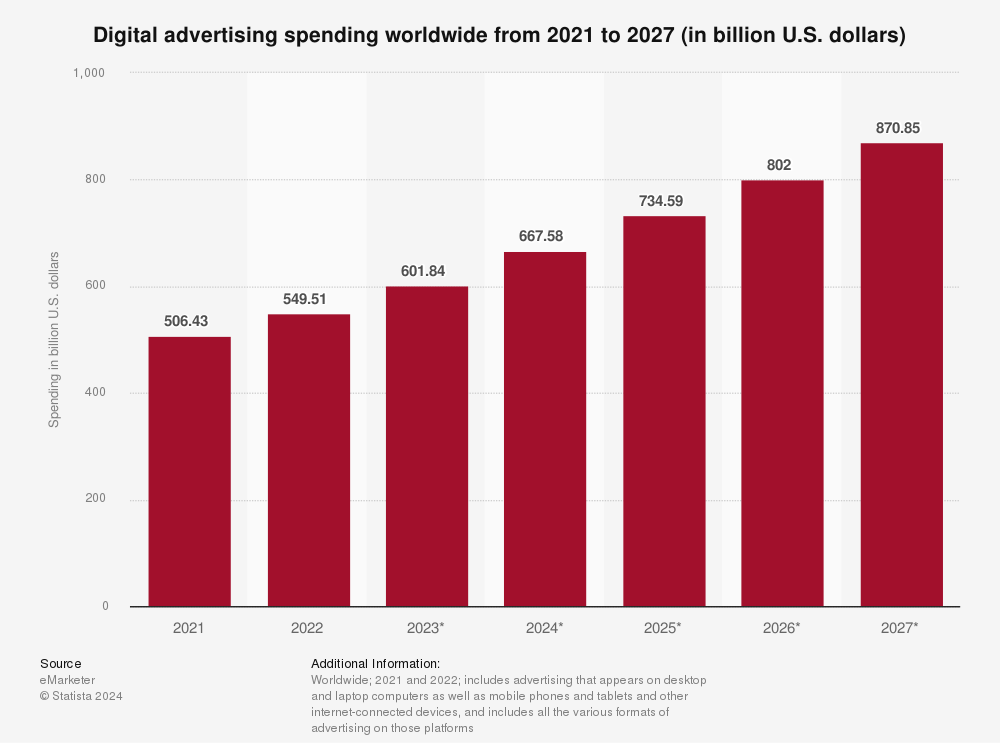
\includegraphics[width=0.8\textwidth]{../figures/eMarketer - Ad Spending.png}
\caption{Global Digital Ad Spending 2021-2027. Image taken from \cite{RefWorks:emarketer2023digital}}
\label{fig:ad-spending}
\end{figure}

Attaining accurate Click-Through Rate (CTR) 
prediction is a necessary first step for Ad persionalization, which is why study of CTR prediction methods have been an extremely active part of 
Machine Learning research over the past through years. Initially, shallow prediction methods such as Logistic Regression, Factorization Machines \citep{RefWorks:rendle2010factorization} and Field-Aware Factorization 
Machines \citep{RefWorks:juan2016field-aware} have been used for CTR prediction. However, these methods have often been shown to be unable to capture the 
higher order feature interactions in the sparse multi-value categorical Ad Marketplace datasets \citep{RefWorks:zhang2021deep}. Since then, Deep Learning methods have been 
shown to show superior predictive ability on these datasets. A number of Deep Learning models have been proposed, each using a
different techniques for feature interaction modelling, ranging from Deep Learning extensions of Factorization Machines
such as DeepFM \citep{RefWorks:guo2017deepfm:}, to novel methods such as AutoInt \citep{RefWorks:song2019autoint}. By employing a
multi-towered neural network architecture, these models are able to capture both low-order and high-order feature interactions in the data,
and therefore tend to achieve supperior predictive performance to their shallow counterparts.

However, irrespective of how well these models perform in a static environments, the reality is that user preferences
and advertisment characteristics are constantly changing. Like most online reccomender systems,
Ad personalization models must be able to adapt to these changes in order to continue to provide accurate predictions 
over the longer period \citep{RefWorks:zheng2018drn:}. This problem necessitates the use
of Reinforcement Learning for Ad personalization.

Reinforcement Learning is a subdomain of Machine Learning in which the goal is for an agent to
learn an optimal policy that maximizes the expected reward in an environment where the
state-action-reward progression can be modelled as a Markov Decision Process
\citep{puterman2014markov}. Early Reinforcement Learning methods involved 
deriving a the transition probabilities for the state-action pairs on the basis of interactions
with the environment and then using Dynamic Programming methods such as the Upper Confidence
Bound RL (UCB-RL) algorithm \citep{RefWorks:auer2008near-optimal} and the
the Thompson Sampling algorithm for Reinforcement Learning \citep{RefWorks:pike-burke2024optimism/thompson}.
However, in cases where the state-action space is too sparce to be
reasonably enumerated, it is often more practical to user a function approximator 
to directly estimate the expacted cumalative reward for each action in each state. This method of Reinfocement
Learning is commonly referred to as Q-learning \citep{RefWorks:watkins1989learning},
and has the advantage of being \emph{model-free}, meaning that
it does not require the agent to have a model of the environment
thereby making it more scalable to large and sparce datasets. In \citep{RefWorks:hornik1989multilayer},
\citep{RefWorks:cybenko1989approximation} and \citep{RefWorks:hornik1990universal} Deep
Neural Networks with activation functions are shown to be universal function approximators
which naturally lead to the incorporation of DNN's in Q-Learning. This has lead to the
development of the Deep Q-Learning Agent, which has been shown to be able to learn optimal
policies in a number of different domains, such as the Atari 2600 game environment \cite{RefWorks:mnih2015human-level}.
Beyond this, Deep Reinforcement Learning has shown promising results in a number
of different aplications, including robot control and computer vision \citep{RefWorks:wang2024deep}.
In the context of Ad personalization, DRL has also be applied to online reccomender systems
such as News article reccomendation \citep{RefWorks:zheng2018drn:} and video
reccomendation on Youtube \citep{RefWorks:chen2019top-k}. In both papers,
the authors show that the DRL agent is able to learn an optimal content reccomendation
policy on the basis of user engagement data. This reveals that there is potential
for applying these methods to the problem of Ad personlization, thereby creating a 
truely adaptive marketing platform.

\subsubsection{Research Question and Contributions}

In this report, I aim to construct a Ad serving system that is truely adaptive and 
personalized to the changing user preferences and advertisment charateristics. In order
to achieve this goal, I will first need to find a suitable Deep Learning Model arcitecture
for CTR prediction, and then incorporating this model as the Q-function approximator in
a Deep Q-Learning algorithm. The key contributions that I make in this report are as follows:

\begin{itemize}
\item I evaluate the performance of five popular Deep Learning models for CTR prediction on three well-known benchmark datasets, Criteo \citep{RefWorks:tien2014display}, KDD12 \citep{RefWorks:aden2012kdd} and Avazu \citep{RefWorks:wang2014click-through}.
\item I construct a novel Deep Reinforcement Learning Frame for Ad personalization, and as a proof-of-concept and evaluate its performance using the KDD12 dataset.
\end {itemize}

\subsubsection{Structure of the Report}

In chapter~\ref{chap:background}, I begin by providing a background introducing the problem
of Click-Through Rate prediction in the context of Ad personalization, and explore the unique challenges posed 
by the typically sparse multi-value categorical datasets that are common in the Ad marketplace. I then 
proceed to review the literature on Deep Learning models for CTR prediction, highlighting
the different techniques that each framework uses to capture the key feature interactions in the data. 
I also review the literature on Deep Reinforcement
Learning, specifically the DRN algorithm introduced by \cite{RefWorks:zheng2018drn:}, which can be analogously
applied to the Ad personalization context. In chapter \ref{chap:deep-ctr-model-evaluation}, I evaluate the performance of different
Deep Learning models for CTR prediction on three well-known benchmark datasets, Criteo \citep{RefWorks:tien2014display}, KDD12 \citep{RefWorks:aden2012kdd} 
and Avazu \citep{RefWorks:wang2014click-through}. In chapter~\ref{chap:deep-rl-for-ad-personalization}, I construct a Deep Reinforcement Learning model for Ad personalization and evaluate its performance
on the same benchmark datasets. Finally, in chapter~\ref{chap:discussion}, I discuss the results of the experiments and provide some concluding remarks.

\chapter{Background}
\label{chap:background}

\section{Deep CTR Prediction}

\subsection{Problem Formulation and Ad Marketplace Data}
\label{sec:problem-formulation-data}

In their respective surveys on the use of Deep Learning methods for CTR prediction, \cite{RefWorks:gu2021ad} 
and \cite{RefWorks:zhang2021deep} outline the problem of CTR prediction as one that essentially boils down to
a binary (click/no-click) classification problem utilizing user/ad-view event level online session records. 
The goal of CTR prediction is to train a function $f$ that takes in a set of ad marketplace 
features $\mathbf{x} \in \mathbb{R}^n$, and maps these to a probability that the user 
will click on the ad in that given context. In other words, $f_{\Theta}: \mathbb{R}^n \rightarrow \mathbb{R}$ such that:

\begin{equation}
\label{eqn:ctr-classifier}
\mathbb{P}(\text{click}| \mathbf{x})
= \mathbb{P}(y = 1 | \mathbf{x})
= \sigma(f_{\Theta}(\mathbf{x}))
\end{equation}

where $y$ is the binary click label, $\Theta$ represents the parameter vector for $f$ and
$\sigma(x)=(1 + e^{-x})^{-1}$ is the sigmoid function. To ease the notation for the rest of the report,
we will use the shorthand $p(y) = \mathbb{P}(y=1 | \mathbf{x})$ formulations in the following
sections. 

An instance of the ad marketplace features $\mathbf{x}$ is typically
recorded at a user/ad impression event level and typically consists of

\begin{itemize}
\item \textbf{User Features:} Features that describe the user, such as User ID, demographic information,
metrics related to the user's past interactions with the platform, etc.
\item \textbf{Ad Features:} Features that describe the ad, such as Ad ID, Advertiser ID and Ad Category.
\item \textbf{Contextual Features:} Features that describe the context in which the ad is being shown, such as
the time of day, the position of the ad on the page and the site on which the ad is being shown.
\end{itemize}

\begin{figure}[h]
\centering
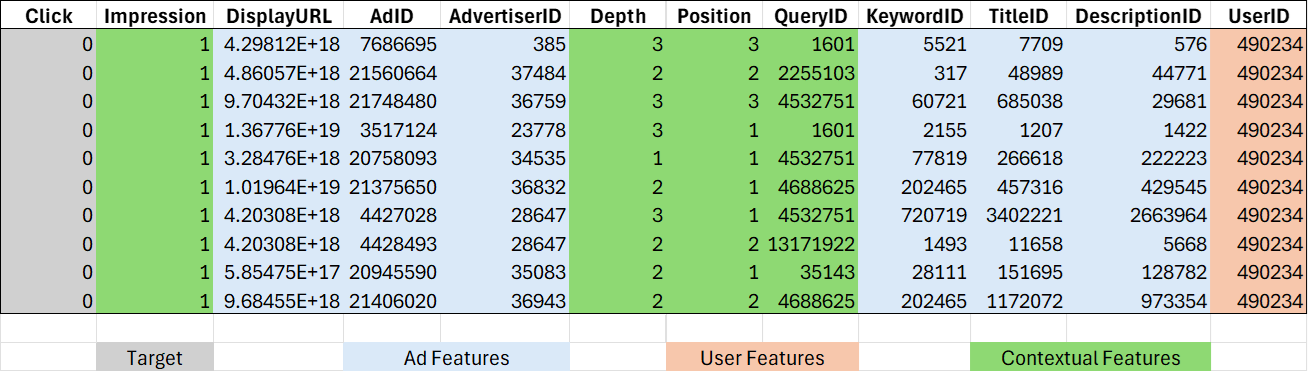
\includegraphics[width=0.8\textwidth]{../figures/kdd12_snapshot.png}
\caption{Snapshot of the KDD12 dataset \cite{RefWorks:aden2012kdd}}
\label{fig:kdd12-snapshot}
\end{figure}

Figure~\ref{fig:kdd12-snapshot} shows a snapshot of the KDD12 dataset, which is a typical example of 
the type of data that is used for CTR prediction.

A defining characteristic for this type of data is that many of the features are multi-value categories with 
a high degree of of cardinality \citep{RefWorks:he2017neural}. In order to user categorical data
in a classifier model, it is common practice to embed the these categorical features
as multidimensional vectors. While the dimensionality of these embeddings can vary amongt the different
sparse categorical features, for the sake of simplicity of notation, below we assume that all sparse categorical feature
embeddings have the same dimensionality, $D$. Let $\mathbf{x_i}^{OH}$ be the one-hot encoded vector
representation of the categiorical feature $x_i$. Then the \emph{embedded} feature vector
$\mathbf{e}_i$ for categorical feature $x_i$ is given by:

\begin{equation}
\label{eqn:cat-embedding}
\begin{split}
\mathbf{e}_i &= \mathbf{B}_i \mathbf{x}_i^{OH}\\
&= \left[\mathbf{b}_{1}^{i}, \ldots, \mathbf{b}_{m_i}^{i} \right] \mathbf{x}_i^{OH} \\
&= \begin{bmatrix}
b_{1,1}^i & \cdots & b_{1 ,C_i}^i\\
\vdots & \ddots & \\
b_{D, 1}^i & \cdots & b_{D, C_i}^i
\end{bmatrix}
\begin{bmatrix}
    0 \\
    \vdots \\
    1 \\
    0\\
    \vdots
\end{bmatrix}
\end{split}
\end{equation}

where $\mathbf{B}_i$ is the embedding matrix for feature $x_i$, whose dimensions are determined
by the chosen embedding dimension $D$ and the cardinality of the feature, $C_i$. Assuming
that value of $x_i$ is equal to the $k$-th value in the one-hot encoding mapping, and that therefore
the $k$-th value in $\mathbf{x}_i^{OH}$ is equal to one, Equation~\ref{eqn:cat-embedding} then simplifies
to

\begin{equation}
    \mathbf{e}_i = \left[e_{i 1}, \ldots, e_{i, D} \right]^{\intercal}
    = \left[b_{1 k}^{i}, b_{2 k}^{i}, \ldots , b_{D k}^{i}\right]^{\intercal} = \mathbf{b}_{k}^{i}
\end{equation}

which is the $k$-th column of the embedding matrix $\mathbf{B}_i$, otherwise referred to as the $k$-th
embedding vector \citep{RefWorks:hancock2020survey}. The processed data $\tilde{\mathbf{x}}$ that then gets fed into the model is 
then composed of a concatenation of all sparse feature embeddigs $\mathbf{e}_i$ and standardized
dense numerical feature values
$z_i = (x_i - \bar{x_i})/\sqrt{Var(x_i)}$:

\begin{equation}
    \begin{split}
    \tilde{\mathbf{x}} &= \left[ \mathbf{e}_1^{\intercal}, \dots , \mathbf{e}_s^{\intercal}, z_{s+1}, \dots , z_{s+d} \right]\\
    &= \left[e_{1, 1}, \ldots, e_{1 ,D}, e_{2, 1}, \ldots , e_{s, D}, z_{s+1}, \ldots, z_{s+d}\right]\\
    &= \left[ \tilde{x}_1, \ldots, \tilde{x}_{\tilde{n}}\right]
    \end{split}
\end{equation}

where $s$ and $d$ are the number of \emph{sparse} categorical features and \emph{dense}
numerical features respectively in $\mathbf{x}$, and $\tilde{n} = D\cdot s + d$
is the resulting dimensionality of $\tilde{\mathbf{x}}$. Again, to ease the notation in the
remainder of the report, we will assume that the prepocessing steps described above
are applied to the data, and all formulaic expressions of the models in the following
section with be expressed in terms of $\tilde{\mathbf{x}} = \{\tilde{x}_j\}_{j=1}^{\tilde{n}}$.

The problem posed by high cardinality is that when $m_i$ is large, the high
sparsity of the one-hot encoded vector $x_i^{OH}$ can make in extremely difficult
for a model to learn the key \emph{implicit} features and patterns present in the
data \citep{RefWorks:gu2021ad}. This is indeed the key challenge in building an
accurate CTR prediction model, and is a key motivating factor as to why Deep Neural
networks have out performed the classical shallow counterparts. This transition will be examined
in more detail in the following section.

\subsection{Shallow CTR Models}
\label{sec:shallow-models}

\subsubsection{Logistic Regression}

The earliest examples of CTR classification models incorporated classical ``shallow'' 
(single layer) statistical regression methods. The most basic example of this was 
the \textbf{Logistic Regression} model, as implemented by \cite{RefWorks:richardson2007predicting} on
advistisment data from the Microsoft Search engine. The LR model
is composed by modelling the \emph{log-odds} (also referred to as the \emph{logit}) 
of a positive binary label as a linear combination
of all of the respective feature values:

\begin{equation}
\label{eqn:lr-model}
f_{\Theta}^{LR}(\tilde{\mathbf{x}}) = \theta_0 + \sum_{j=1}^{\tilde{n}}\theta_j \tilde{x}_j
\end{equation}

where $f_{\Theta}^{LR}: \mathbb{R}^n \rightarrow \mathbb{R}$ represents the Logistic regression
model parametized by $\Theta = (\theta_0, \ldots, \theta_{\tilde{n}})$. The benefits of the LR
model are that due to its simplicity and low number of parameters, it is relatively easy to
train in computational terms and also relatively easy to deploy \citep{RefWorks:zhang2021deep}.
Howevever, the formulation in equation~\ref{eqn:lr-model} reveals that the LR model does not explicitly 
account for \emph{feature interactions}.
As outlined in section~\ref{sec:problem-formulation-data}, the categorical features tend to have a
high cardinality, resulting in highly sparse feature embeddings. Many of the of the important patterns
for CTR prediction are therefore likely to be expressed in terms of \emph{combinations of features}
rather then the individual feature values themselves. For example, a user's tendancy to
click on a given advertisment is likely to by influenced by the \emph{combination} of the category
of good or service the given advertisment is trying to sell (e.g. premium fashion retail, travel, electronics et. cetera)
and the demographic/socio-economic category that the given user falls into (e.g. university student, young professional, retiree).
These features combinations (and the corresponding combination of respective field values 
in the preprocessed feature vector $\tilde{\mathbf{x}}$) are commonly referred to in
the literature as \emph{cross-features} \citep{RefWorks:zhang2023memonet:} or more commonly
\emph{feature interactions} \citep{RefWorks:cheng2016wide,RefWorks:xiao2017attentional,RefWorks:song2019autoint}.

Whilst it is possible to incorporate feature interactions in an LR model through feature
engineering, this quickly becomes infeasible for large sparse datasets. A number of techniques
have been developed to automate the necessary feature engineering steps for this, either by
implicitly assigning a weight to all second order feature interactions \citep{RefWorks:chang2010training}
or by utilizing Gradient Boosted Decision Trees to pick out the key interactions \citep{RefWorks:cheng2014gradient}.
Unfortunately, the prior still tends to exhibit poor performance with sparse data, 
whereas the fact that the Gradient Boosting algorithm for the latter is difficult to paralellize
makes this solution difficult to scale in many applications in practice \citep{RefWorks:zhang2021deep}.

\subsubsection{Factorization Machines}

\textbf{Factorization Machines} first proposed by \cite{RefWorks:rendle2010factorization} can 
be thought of as an extension of the Logistic Regression framework in equation~\ref{eqn:lr-model}
with additional terms that explicitly account for the interactions between different features.
Its relative simplicity and computational scalability has made it a widely popular framework
for CTR modelling \citep{RefWorks:gu2021ad}. 
A 2-way (maximum feature interaction degree of 2) Factorization Machine model is formulated as:

\begin{equation}
\label{eqn:fm-2way}
f_{\Theta}^{FM^2}(\tilde{\mathbf{x}}) = \theta_0 + \sum_{j=1}^{\tilde{n}} \theta_{j} \tilde{x}_j
+ \sum_{j=1}^{\tilde{n}} \sum_{k=j+1}^{\tilde{n}} \langle \mathbf{v}_j , \mathbf{v}_k \rangle \tilde{x}_j \tilde{x}_k
\end{equation}

where $\langle \cdot , \cdot \rangle$ represents the inner product between two vectors, the final
interaction term above is parametized by $\mathbf{V} \in \mathbb{R}^{\tilde{n} \times F}$. Each
row $\mathbf{v}_j$ of $\mathbf{V}$ represents the $j$-th feature in $\tilde{\mathbf{x}}$ in terms
of $F$ latent factors. The factorization matrix $\mathbf{V}$ is typically fitted by optimizing
the binary cross-entropy loss function by means of Stochastic Gradient Descent. It is 
intutive to see that $\mathbf{V}$ will be fitted such that if the interaction
between feature $j$ and $k$ have a positive impact on $p(y)$, then $j$-th and 
$k$-th rows of $\mathbf{V}$ will have positive inner products (and vice versa) \citep{RefWorks:zhang2021deep}.

\cite{RefWorks:rendle2010factorization} shows that although direct evaluation
of equation~\ref{eqn:fm-2way} would appear to have a complexity of $O(F \tilde{n}^2)$, the 2-way
FM model in fact scales linearly in $\tilde{n}$ and $F$:

\begin{lemma}
\label{lemma:fm-linearity}
The model equation of a 2-way factorization machine (eq.~\ref{eqn:fm-2way}) can
be computed in linear time $O(F\tilde{n})$.
\end{lemma}

\begin{proof}
\label{prf:fm-linearity}

Due to the factorization of the pairwise interactions, there is no model
parameter that directly depends on two features $(j,k)$. This means that
pairwise interactions can be reformulated as such

\begin{align*}
    &\sum_{j=1}^{\tilde{n}} \sum_{k=j+1}^{\tilde{n}} \langle \mathbf{v}_j , \mathbf{v}_k \rangle \tilde{x}_j \tilde{x}_k \\
    &= \sum_{j=1}^{\tilde{n}} \sum_{k=j+1}^{\tilde{n}} 
    \sum_{f=1}^{F}v_{j,f} v_{k,f}\tilde{x}_j \tilde{x}_k \\
    &= \frac{1}{2} \left( \sum_{j=1}^{\tilde{n}} \sum_{k=1}^{\tilde{n}}
    \sum_{f=1}^{F} v_{j,f} v_{k,f} \tilde{x}_j \tilde{x}_k -
    \sum_{j=1}^{\tilde{n}} \sum_{f=1}^{F}v_{j,f} v_{j,f} \tilde{x}_j \tilde{x}_j \right)\\
    &=\frac{1}{2}\sum_{f=1}^{F} \left( \sum_{j=1}^{\tilde{n}}v_{j,f} \tilde{x}_j
    \sum_{k=1}^{\tilde{n}} v_{k,f} \tilde{x}_k - \sum_{j=1}^{\tilde{n}}
    v_{j,f}^2 \tilde{x}_j^2 \right)\\
    &= \frac{1}{2}\sum_{f=1}^{F} \left( \left(\sum_{j=1}^{\tilde{n}}v_{j,f} \tilde{x}_j\right)^2
    - \sum_{j=1}^{\tilde{n}} v_{j,f}^2 \tilde{x}_j^2 \right)
\end{align*}

The complexity of the final line above is $O(F\tilde{n})$, and hence the FM formulation
as per equation~\ref{eqn:fm-2way} scales linearly in $F$ and $\tilde{n}$.
\end{proof}

This quality greatly simplifies the computational complexity of scaling the FM model to larger
datasets with a more sparse categorical features. Morever, the Factorization Machine framework
can be generalized to degree $R$ (i.e. up to any limit of feature interation order) as follows:

\begin{multline}
\label{eqn:fm-rway}
f_{\Theta}^{FM^R} = \theta_0 + \sum_{j=1}^{\tilde{n}} \theta_{j} \tilde{x}_{j}
+ \sum_{r=1}^{R} \sum_{j_1=1}^{\tilde{n}} \cdots \sum_{j_r = j_{r-1} + 1}^{\tilde{n}}
\left( \prod_{k=1}^{r} \tilde{x}_{j_k} \right)
\left( \sum_{f = 1}^{F_r} \prod_{k=1}^{r} v_{j_k, f}^{(r)}\right)
\end{multline}

The FM framework therefore provides an intuitive and computationally scalable method to
account for key feature interactions without the need of extensive feature engineering. Extensions
and improvements to FM have been proposed, most notably in the form of
the Field-Aware Factorization Machine (FFM) framework by \cite{RefWorks:juan2016field-aware},
which only acounts for intereactions between features of different fields 
(in otherwords, it ignores the interaction between $\tilde{x}_j$ and $\tilde{x}_k$ if
both are componets of embedding vector $mathbf{e}_i$ for some categorical feature $x_i$)
as well as Gradient Boosted Factorization Machines \citep{RefWorks:cheng2014gradient}, 
which again aims to augment the FM framework by means of the Gradient Boosting algorithm.

\subsection{Introducing MLP's in CTR prediction}

Despite the advantages of the FM framework, a setback of the formulation in equation~\ref{eqn:fm-rway}
is that the framework grows highly compex and overparametized for higher values of $R$.
As a consequence, only the 2-way FM framework as per equation~\ref{eqn:fm-2way} tends to be
implemented in practice, meaning that the FM model alone is practically insufficient for capturing
feature interactions of order $>>2$ \citep{RefWorks:guo2017deepfm:}. Deep Neural Networks
present a powerful alternative for addressing this shortcoming. Neural networks benefit from
being universal function approximators \citep{RefWorks:cybenko1989approximation} and from the
fact that neural network batch training is paralellizable by means of GPU accelerated computation.
This has lead to the successfull application of Deep Learning algorithms across multiple fields
such as Natural Language Processing and Image classification 
\citep{RefWorks:he2016deep,RefWorks:krizhevsky2017imagenet,RefWorks:lecun1998gradient-based}. 
These factors and successes showed that DNN's have the potential to extract informative
feature representations from highly sparse and abstract data, and as a consequence,
the application of DNN's in CTR prediction started recieving attention in the mid-2010's.

The \textbf{Multilayer Perceptron} (MLP) \label{ref:mlp} is the most elementary type of Deep Neural Network
\citep{RefWorks:webster2024week}. In general, a MLP with $L$ hidden layers is formulated as such:

\begin{align}
\label{eqn:mlp}
\mathbf{h}^{(0)} &:= \tilde{\mathbf{x}} \\
\mathbf{h}^{(l)} &= \phi_{l} \left( \mathbf{W}^{(l-1)} + \mathbf{b}^{(l-1)} \right), l = 1, \ldots, L \\
\hat{y} &= \phi_{out} \left( \mathbf{w}^{(L)} \mathbf{h}^{(L)} + b^{(L)} \right)
\end{align}

where $\mathbf{W}^{(k)} \in \mathbb{R}^{n_{l+1} \times n_l } $, $\mathbf{b}^{(k)} \in \mathbb{R}^{n_{l+1}}$,
$\mathbf{h}^{(l)} \in \mathbb{R}^{n_l}$, $n_0 = \tilde{n}$, $n_l$ is the number of hidden
units in layer $l$ and $\phi_{l}$ is the activation function for layer $l$, 
When rearranged in the form of equation~\ref{eqn:ctr-classifier}, the above becomes:

\begin{equation}
\label{eqn:mlp-2}
f_{\Theta}^{MLP}(\tilde{\mathbf{x}}) = \psi_{out} \left( \psi_{L} \left( \cdots \psi_{1} \left( 
    \tilde{\mathbf{x}} \right) \cdots \right) \right)
\end{equation}

where each function $\psi_{l}$ represents the affine transformation and element-wise activation
operation for layer $l$. MLPs can be thought of as an acyclic graph, as displayed in
Figure~\ref{fig:mlp}. The data $\tilde{\mathbf{x}}$ first gets fed through the
\emph{input layer}, then gets processed by multiple \emph{hidden layers} that include
a series of affine transfromations followed by activation functions, before the final
result is produced by the \emph{output layer}.

\begin{figure}[h]
    \centering
    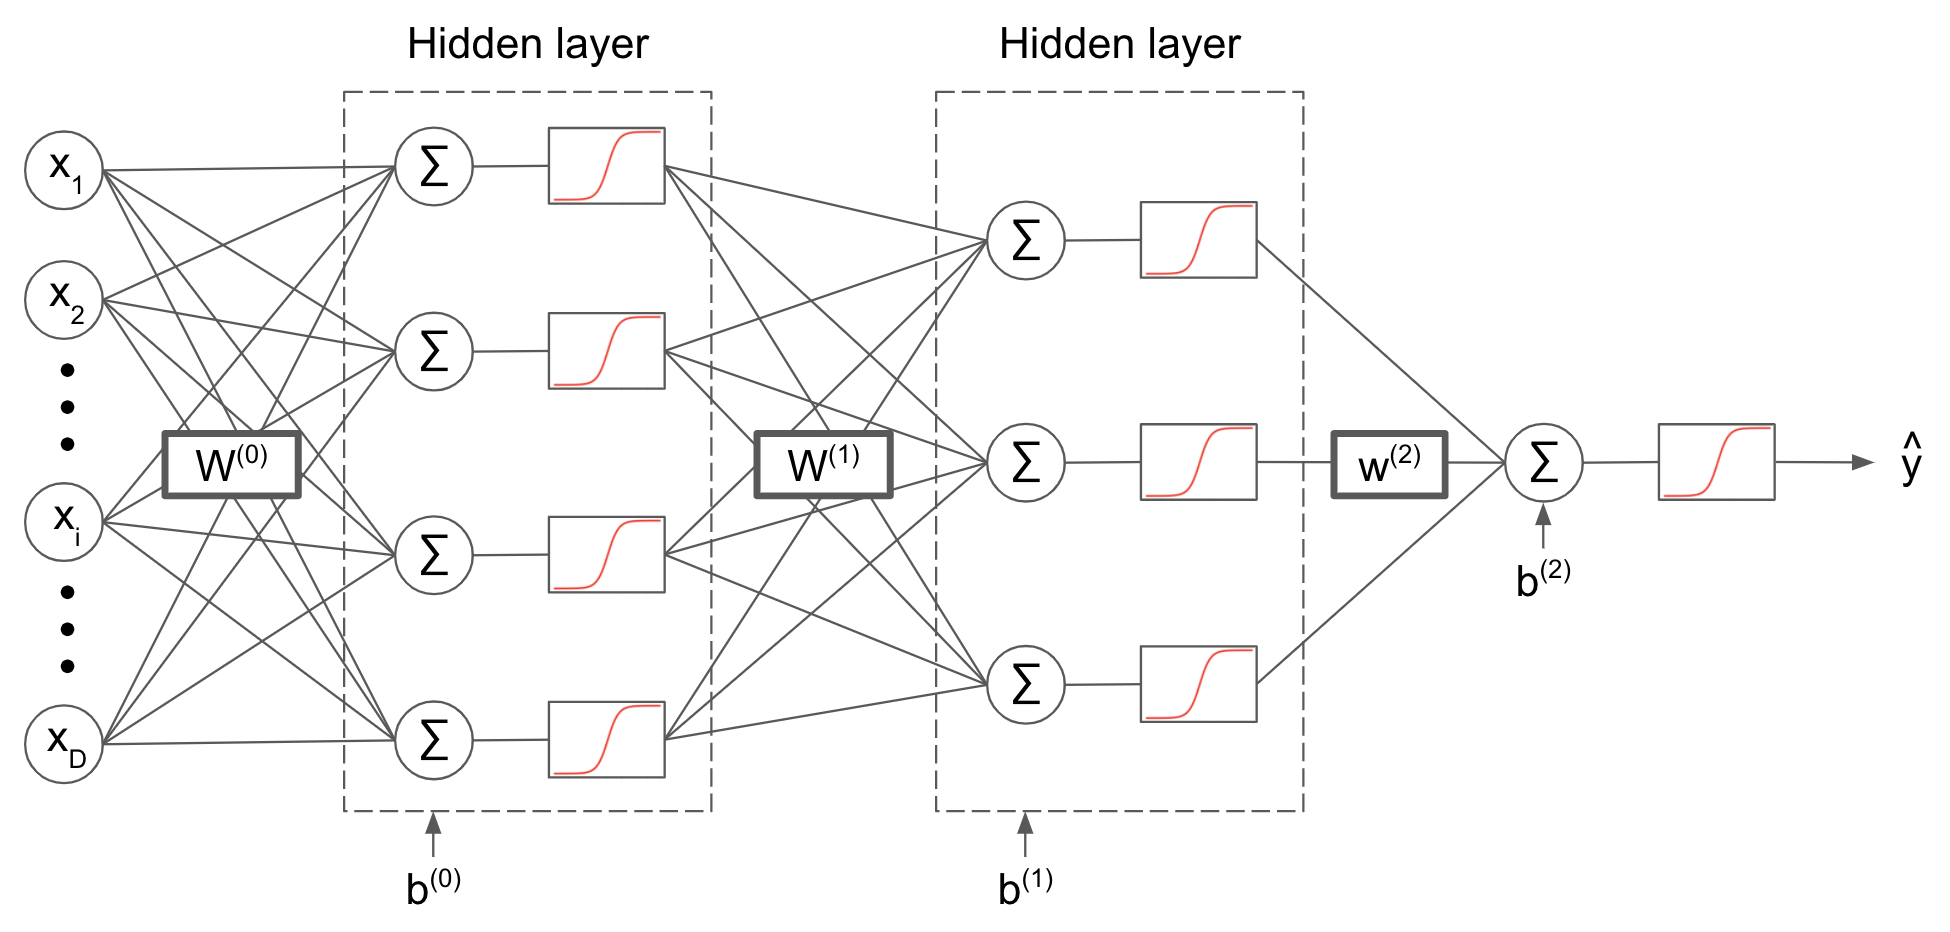
\includegraphics[width=0.8\textwidth]{../figures/ann_two_hidden_layers.png}
    \caption{Multilayer Perceptron with two hidden layer. Taken from \citep{RefWorks:webster2024week}}
    \label{fig:mlp}
\end{figure}

Figure~\ref{fig:mlp} demonstrates the potential that DNN's have for modelling higher order feature
interactions. By training the network by means of Stochastic Gradient Descent, it should be
possible to calculate the appropriate weight ($\mathbf{W}_l$) and bias ($\mathbf{b}_l$) parameters
in order capture the relevant high-order feature patterns in the data. As such, many CTR
modelling frameworks have been developed that use Deep Learning techniques to build upon and
imporved the previously discussed classical methods by incorporating Deep Neural Networks such
as the ML in the model architecture \citep{RefWorks:zhang2021deep}.

\subsection{Single vs Dual Tower Architectures}

Before moving on to DNN enhanced CTR models in section~\ref{sec:mlp-enhanced-models}
it is worth briefly discussing the difference between \textbf{Single-Tower}
models and \textbf{Dual-Tower} architecture models. Single Towel models place
all layers successively in the architecture, and can generally be formulated
as in equation~\ref{eqn:mlp-2}. Since all feature inputs are passed through
the same set of successive affine transformations and activations, Single Tower
models are usually able to capture higher order feature interactions, but the signal
from the low-order interactions tend to be lost \citep{RefWorks:zhang2021deep}.
The FNN \citep{RefWorks:zhang2016deep}, FGCNN
\citep{RefWorks:liu2019feature} and PNN \citep{RefWorks:qu2016product-based} models covered in the subsections 
\ref{sec:mlp-enhanced-models} and \ref{sec:feature-operator-models}
are examples of Single Tower models.

In order to avoid diluting the signal from the lower order feature interactions, many architectures
adopt a Dual Tower architecture, as shown on the right-hand side of
Figure~\ref{fig:single-dual-models}. A separate \textbf{Feature Interaction Layer}
is placed paralelly to the DNN, and the final output is composed of a weighted sum
of the feature interaction and DNN outputs. With this architecture, the feature interaction
layer is usually dedicated to capturing the important lower order feature interaction signals,
whereas the DNN acts as a \emph{residual network} for capturing any meaningful signals that may
be missing. As a result, Dual Tower networks tend to benefit form better training stability and
better performance \citep{RefWorks:zhang2021deep}.

\begin{figure}[h]
    \centering
    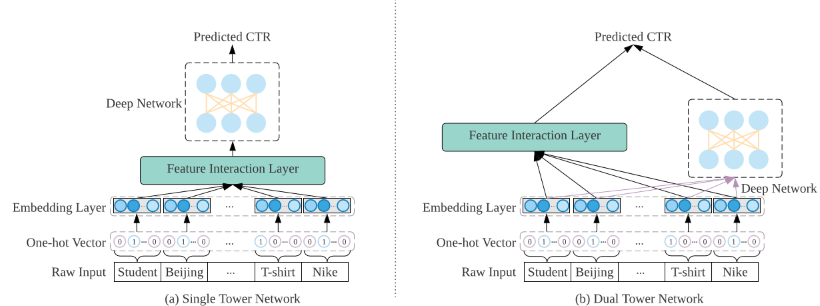
\includegraphics[width=\textwidth]{../figures/single_dual_dnn.png}
    \caption{Single vs Dual Architecture Networks. Source: \citep{RefWorks:zhang2021deep}}
    \label{fig:single-dual-models}
\end{figure}

\subsection{DNN Enhanced CTR models}
\label{sec:mlp-enhanced-models}

\subsubsection{Factorization-machine Supported Neural Networks}

One of the earliest example of the use of Deep Neural Networks being used to enhance existing
CTR modeling methods is the \textbf{Factorization-machine Supported Neural Network} (FNN)
\citep{RefWorks:zhang2016deep}. The FNN model is a Single Tower model that works by pretraining
a 2-way Factorization Machine model as in equation~\ref{eqn:fm-2way} on the concatenated
one-hot encoded categorical feature vectors, and then using the feature interaction vectors and
weights as the embedding matrix.

Below we start with the concatenated one-hot encoded categorical feature vector:
\begin{align*}
    \dot{\mathbf{x}} &= \left[\mathbf{x}_1^{OH}, \ldots, \mathbf{x}_n^{OH} \right]\\
    f_{\Theta}^{FM^2} &= \theta_0 + \sum_{j=1}^{\dot{n}} \theta_j \dot{x}_j +
    \sum_{j=1}^{\dot{n}} \sum_{k=j+1}^{\dot{n}}
    \langle \mathbf{v}_j, \mathbf{v}_k \rangle \dot{x}_j \dot{x}_k
\end{align*}

Using the weights
and biases from $\Theta = (\theta_0, \theta_1, \ldots , \theta_{\dot{n}}, \mathbf{v}_1, \ldots, \mathbf{v}_{\dot{n}})$,
the preprocessed MLP input is calculated as follows:

\begin{equation*}
\tilde{\mathbf{x}} = \left[\theta_0, \mathbf{e}_1^{\intercal}, \mathbf{e}_2^{\intercal}, \ldots, \mathbf{e}_s^{\intercal}\right]
\end{equation*}

where each embedding vector $\mathbf{e}_i$ is defined as the concatination of
the weight ($\theta_i$) and FM interaction vector ($\mathbf{v}_i$) corresponding to feature
$i$ in $\dot{\mathbf{x}}$:
\begin{equation*}
    \mathbf{e}_i = \left[\theta_i, \mathbf{v}_i^{\intercal}\right]
\end{equation*}

The above can alternatively also be recovered from equation~\ref{eqn:cat-embedding} by
setting the embedding matrix $\mathbf{B}_i$ to a $(F+1) \times C_i$ matrix with the following
values

\begin{equation*}
\mathbf{B}_i = \begin{bmatrix}
    b_{1,1}^i & \cdots & b_{1 ,C_i}^i\\
    \vdots & \ddots & \\
    b_{F+1, 1}^i & \cdots & b_{F+1, C_i}^i
    \end{bmatrix}
= \begin{bmatrix}
    \theta_i & \cdots & \theta_i\\
    v_{1}^1 & \cdots & v_{C_i}^1 \\
    \vdots & \ddots & \\
    v_{1}^{F}& \cdots & v_{C_i}^{F}
    \end{bmatrix}
\end{equation*}

Figure~\ref{fig:fnn} portrays the structure of this model as it was presented in the original
paper by \cite{RefWorks:zhang2016deep}.

\begin{figure}[h]
    \centering
    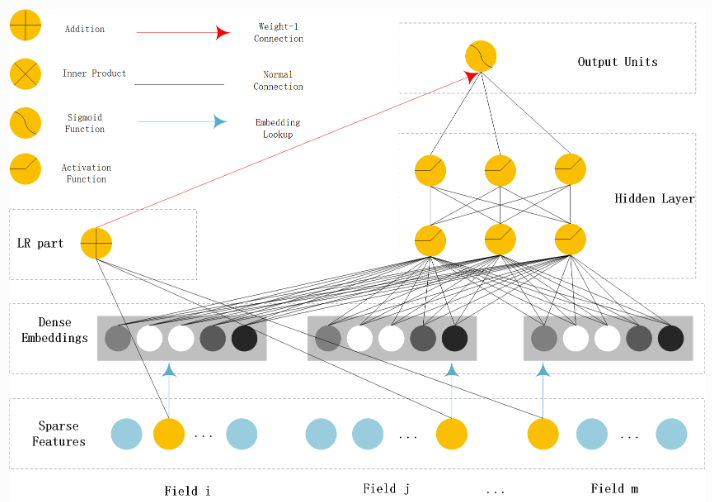
\includegraphics[width=0.8\textwidth]{../figures/fnn.png}
    \caption{FNN model architecture. Source: \citep{RefWorks:zhang2016deep}}
    \label{fig:fnn}
\end{figure}

By incorporating the FM model feature interaction vectors in the embedding layer
before the DNN, the FNN model is able to leverage the FM model's strength in
interaction identification. The FNN model then leverages a MLP network
to capture the higher order interaction signals much more efficiently than would
have been feasibly possible when relying ownly on FM. Because of this, comprehensive
experiments carried out by \cite{RefWorks:zhang2016deep} confirmed that FNN
has superior CTR estimation performance than both LR and FM.

However \cite{RefWorks:guo2017deepfm:} and \cite{RefWorks:zhang2021deep} find that
due to its Single Tower architecture, lower-order feature interaction signals tend
to be lost in the network. \cite{RefWorks:guo2017deepfm:} further found that
the FM pretraining step described above represents a significant overhead in
terms of training efficiency. In the next subsections, we will see how the Wide \& Deep
and DeepFM models aim to solve for these issues.

\subsubsection{Wide and Deep}

The \textbf{Wide and Deep} (W\&D) model was developed by \cite{RefWorks:cheng2016wide}.

\begin{equation}
    \label{eqn:wdl}
    f_{\Theta}^{W\&D} = \theta_0 + \sum_{k=1}^{\hat{n}} \theta_k \hat{\mathbf{x}}_k
    + f_{\Phi}^{MLP}(\tilde{\mathbf{x}})
\end{equation}

\begin{figure}[h]
\centering
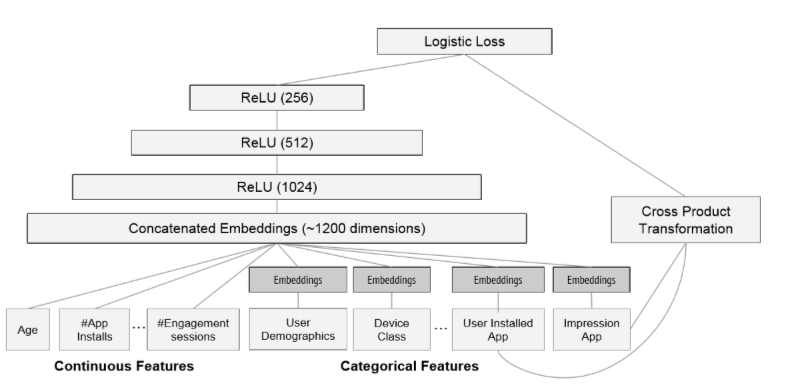
\includegraphics[width = 0.8\textwidth]{../figures/wdl.png}
\caption{Wide and Deep Model, as illustrated in \citep{RefWorks:shen2017deepctr:}}
\label{fig:wdl}
\end{figure}

Figure~\ref{fig:wdl} reveals that the W\&D model is composed with a Dual-Tower Architecture,
with a Deep Component and a Wide Component (shown on the left and right hand sides of Figure~\ref{fig:wdl}
respectively). The Deep Component is composed of a MLP with multiple hidden layers, each
with the Rectified Linear Unit (ReLU) activation function. The Wide Component is formulated
by the first two terms in equation~\ref{eqn:wdl}, and is composed of a simple linear transformation
of the input features. The key aspect of the Wide Component is the fact that the 
linear transformation is not simply applied to the preprocessed features $\tilde{x}$,
but instead to these concatinated with a set of cross-product transformed features. In
other words:

\begin{equation}
\label{eqn:wdl-cross-product}
\hat{\mathbf{x}} = [\tilde{\mathbf{x}}, \upsilon_1({\tilde{\mathbf{x}}}),\ldots , \upsilon_P({\tilde{\mathbf{x}}})]
\end{equation}

Where $\upsilon_k({\tilde{\mathbf{x}}}) = \prod_{j=1}^{\tilde{n}}\tilde{x}_j^{c_{kj}}$
and $c_{kj} \in \{ 0, 1 \}$.

Consequentially of equation~\ref{eqn:wdl-cross-product}, the Wide Component \emph{memorizes}
the key feature interations that are defined by the specific \emph{cross-product transformations}
($\upsilon_{k}(\tilde{\mathbf{x}})$) \citep{RefWorks:cheng2016wide}. Meanwhile, the Deep Component captures any residual
signals that may not have been explicitly included in the manually defined cross-product transformations
\citep{RefWorks:zhang2021deep}. In this sense, the W\&D model overcomes the
shortcomings of the FNN model, by having dedicated pathways in the archtecture
for higher and lower order feature interactions. However, the downside
of W\&D is the fact that the feature interactions in the Wide component
need to be manually incorporated by defining the cross-product transformation
functions $\{\upsilon_k(x)\}_{k=1}^{P}$. This means that there is a significant
feature engineering component that would be necessary to use this model effectively. 

\subsubsection{DeepFM}

The \textbf{DeepFM} model was developed by \cite{RefWorks:guo2017deepfm:} in order
to address the shortcomings of the FNN and W\&D models mentioned in this section, as 
well as those of the PNN model which will be covered in section~\ref{sec:feature-operator-models}.
Similarly to the W\&D model, the DeepFM network two components arranged as a Dual Tower
architecture, as visualized in Figure~\ref{fig:deepfm}.

\begin{figure}[h]
    \centering
    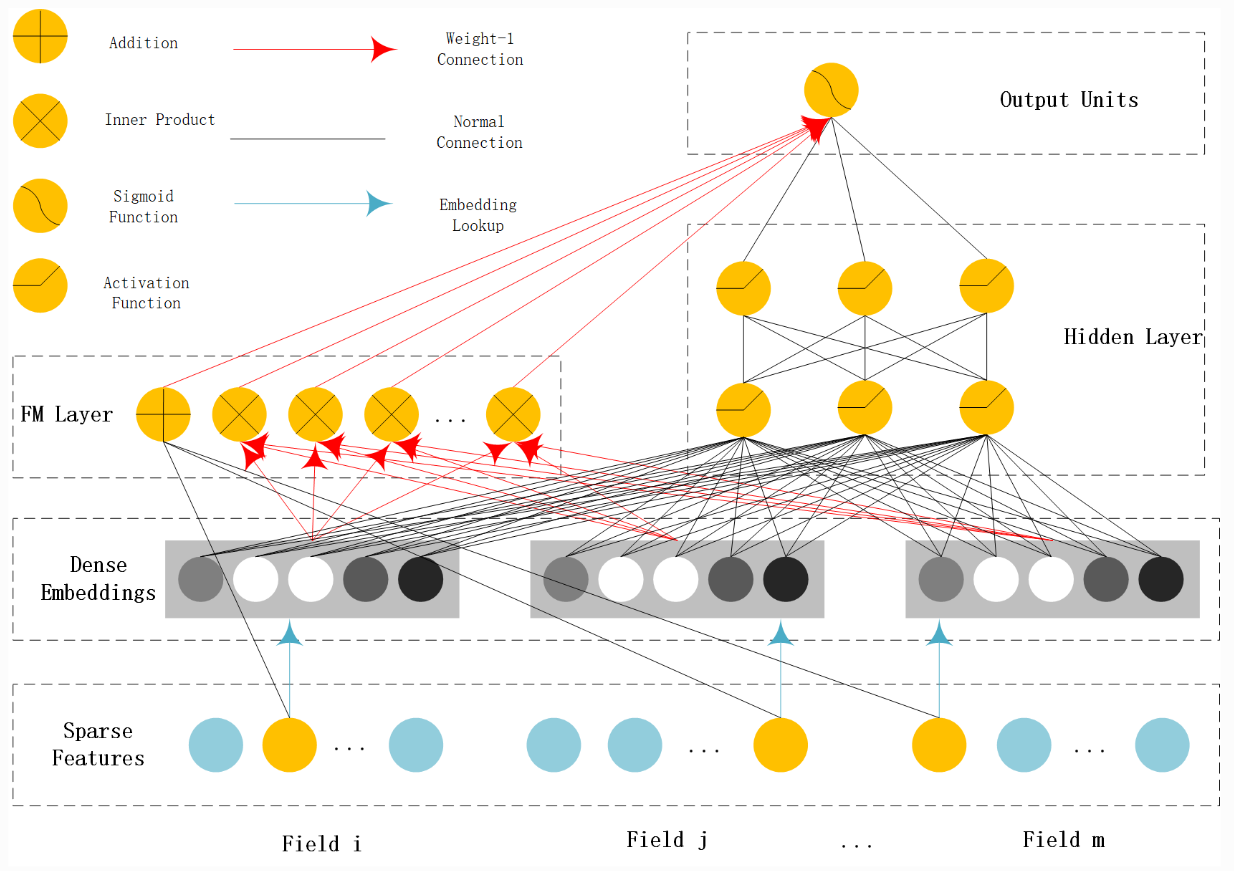
\includegraphics[width=0.8\textwidth]{../figures/dfm.png}
    \caption{DeepFM network architecture. Source: \citep{RefWorks:shen2017deepctr:}}
    \label{fig:deepfm}
\end{figure}

The \emph{FM component} effectively replaces the Wide component in the W\&D model. It consists
of a 2-way Factorization Machine layer that models pairwise feature interactions between the
different fields of $\tilde{\mathbf{x}}$ as inner products of the respective feature latent
vectors $\mathbf{v}_j$ \citep{RefWorks:guo2017deepfm:}. Due to the linear scalability of
the FM discussed in section~\ref{sec:shallow-models}, the FM component can effectively
capture important order-2 feature interactions automatically, without the need to manually
define cross-product functions as in the case of the W\&D model.

Meanwhile, the \emph{Deep component} fulfills a similar purpose as in the case of the W\&D
model. The deep component is a MLP network that takes the feature embedding vector $\tilde{\mathbf{x}}$
as inputs, and learns the higher-order feature interactions that cannot by captured by the
2-way FM component. Like with the W\&D model, the Deep component acts as a residual network
for capturing signals that we ommitted by the FM component. The DeepFM model can therefore
be formulated as in equation~\ref{eqn:deepfm}.

\begin{equation}\label{eqn:deepfm}
    f_{\Theta}^{DeepFM} = f_{\Phi}^{FM^2}(\tilde{\mathbf{x}}) + f_{\Omega}^{MLP}(\tilde{\mathbf{x}})
\end{equation}

A notable difference
in the Deep components between the W\&D and DeepFM models are in the construction of the
embedding layers that preprocess the input to the MLP. In DeepFM, the latent feature vectors
($\mathbf{V}$) are trainable network weights that are derived during SGD optimization in the FM
component. For every successive step in the model training, the learned latent feature vectors
are used in the embedding layer that preprocesses that raw input features before the MLP of 
the Deep component (see Figure~\ref{fig:deepfm-embedding}). This is similar to how the feature embeddings were derived in the FNN model
\citep{RefWorks:zhang2016deep}, except for fact the FM layer is included in the overall learning
architecture of the model. This elimitates the need to pretrain the FM model, thereby allowing
for the FM latent feature vectors to by learned concurrently during the overall DeepFM model
training procedure \citep{RefWorks:guo2017deepfm:}.

\begin{figure}[h]
    \centering
    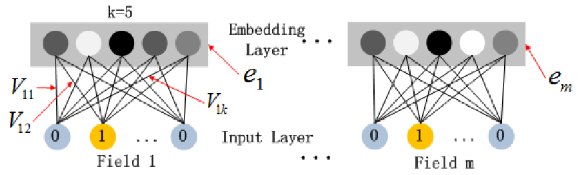
\includegraphics[width=0.8\textwidth]{../figures/deepfm_embedding.png}
    \caption{The embedding layer of the Deep Component in the DeepFM model. Source: \citep{RefWorks:guo2017deepfm:}}
    \label{fig:deepfm-embedding}
\end{figure}

The key benefits of the DeepFM model are threefold. Firstly, we have already mentioned above
that the fact that the FM model is incorporated directly into the model architecture eliminates
the need to pretrain the FM latent feature vectors, thereby eliminating the computational overhead
that is neccessary for this in the case of FNN \citep{RefWorks:zhang2016deep}. Secondly,
the Dual Tower architecture allows the model to simultaneously learn both low as well as high
order feature interactions. Thirdly, the previously discussed computational efficiency of the
FM model means that DeepFM is relatively scalable in terms of the number of features and the size of
the latent embedding space, especially in comparison to the Product based Neural Network
(PNN) models \citep{RefWorks:qu2016product-based}, which will be covered in section \ref{sec:feature-operator-models}.

\subsection{Feature Interaction Operator Models}
\label{sec:feature-operator-models}

MLPs have been proven to be universal function approximators, meaning that any function can be
can be sufficiently approximated with a larger enough MLP \citep{RefWorks:hornik1989multilayer,RefWorks:cybenko1989approximation,RefWorks:hornik1990universal}.
However, \cite{RefWorks:shalev-shwartz2017failures} found that for complex problems where the true target function
is actually a larger set of uncorrelated solution functions, Deep Neural Networks suffer from
an \emph{insensitive gradient issue} during gradient descent optimization. \cite{RefWorks:shalev-shwartz2017failures}
show that when the target function is a set of uncorrelated functions, the variance of the gradient
with respect to the target decreases linearly with respect to the number of functions that make up the target.
The decrease in this variance has the effect of decreasing the correlation between the gratient
and the target, causing the optimization of the DNN to fail. \cite{RefWorks:qu2018product-based}
argues that since the target function for the CTR classification task typically consists of a
set of uncorrilated if-then classifiers on the basis sparse categorical features, the insensitive
gradient issue is likely to be prevalent in cases where MLPs are relied upon directly
to detect the key feature interactions in sparse CTR classification data.

The above justifies the design of specific layers and architectures that explicitly detect important
feature interactions in the data. In this section, we discuss \textbf{Feature Interaction Operators},
which are deep learning layers that were developed specifically to assist the DNN in its capacity
to learn higher feature interactions \citep{RefWorks:zhang2021deep}. The three different type of Feature Interaction
Operators that are discussed in this section are Product Operators, Convolutional Operators
and Attention Operators.

\subsubsection{Product Operators models}

\textbf{Product Operator} networks are neural networks that include layers with inner or outer
product operations in order to explicitly model feature interactions \citep{RefWorks:zhang2021deep}.
The \textbf{Product-bassed Neural Network} (PNN) introduced the concept of product operator models
as it includes a product layer between the embedding layer and the MLP in order to model second
order feature interactions in the data. All of this is arranged as a Single Tower architecture, as shown
in Figure~\ref{fig:pnn}.

\begin{figure}[h]
    \centering
    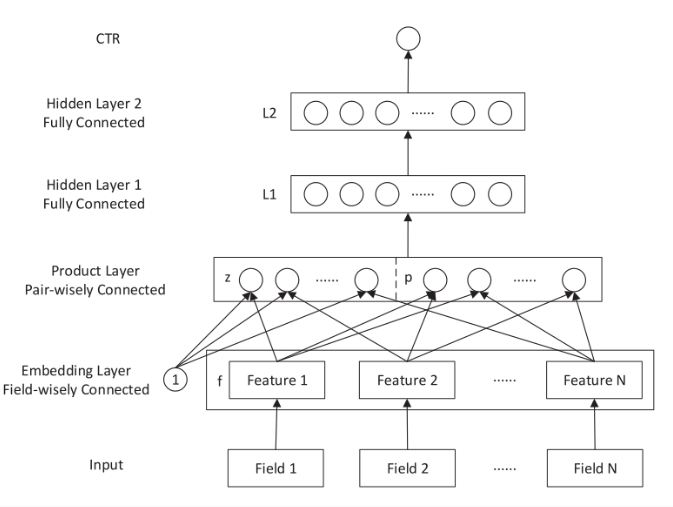
\includegraphics[width=0.8\textwidth]{../figures/pnn.png}
    \caption{Product-based Neural Network. Source: \citep{RefWorks:qu2016product-based}.}
    \label{fig:pnn}
\end{figure}

The key defining component of the PNN is the \emph{Product Layer}. Each embedding field $\mathbf{e}_i$
in the preceding embedding layer is pair-wisely connected to each of the other fields and a ``1''
constant signal. The output of the product signal can then be broken out into two parts:

\begin{itemize}
    \item Virtue to the constant ``1'' signal, the first part is simply a vector $\mathbf{z}$ that consists of a concatenation
    of all of the field embeddings. In other words $\mathbf{z} = \tilde{\mathbf{x}}$.
    \item A second-order interaction vector, $\mathbf{p} = \{p_{i,j}\}\text{ where } i,j = 1, \ldots, n$, where each element
    $p_{i,j} = g(\mathbf{e}_i, \mathbf{e}_j)$ defines a pairwise field interaction.
\end{itemize}

In their initial paper, \cite{RefWorks:qu2016product-based} proposed two variants of the PNN model, the Inner Product Based Neural Network
and the Outer Product Based Neural Network, differentiated by whether $g$ is the Inner or Outer
product operation respectively. The $\mathbf{z}$ and $\mathbf{p}$ vectors are then both
projected to $\mathbb{R}^{D^1}$ space (the input dimension of the MLP network) by meant
of trainable weight matrices, $W_z$ and $W_p$. The input to the MLP network is then the
sum of the two resulting vectors and a bias vector $\mathbf{b}_1$. The formulation
for the PNN network is summarized in equation~\ref{eqn:pnn}.

\begin{equation}\label{eqn:pnn}
    f_{\Theta}^{PNN}(\tilde{\mathbf{x}}) = f_{\Phi}^{MLP}(W_z \tilde{\mathbf{x}} + W_p \{g(\mathbf{e}_i, \mathbf{e}_j)\}_{i,j=1}^{n} + \mathbf{b}_1)
\end{equation}

The inclusion of the product layer in the PNN model automatically incorporates second order field-wise
interactions as inputs to the MLP by means of inner and outer products, thereby partially alleviating
the previously mentioned insensitive gradient issue. \cite{RefWorks:qu2016product-based} found that
as a result of this, the PNN models outperformed LR, FM, FNN and the CCPM models in terms of Log Loss
and AUC. However, a major disadvantage of the product layer operations is the computational time complexity,
which increases quadratically with the number of fields and the embedding dimension. In order to alleviate
this, \cite{RefWorks:qu2016product-based} implement simplified versions of the inner and outer product
computations (in which some neurons are eliminated in the inner product, and the result for the outer product
is compressed for all fields at once), but even then the PNN models are still tend to be less computational
than its peers. Furthermore, since the PNN model leverages a Single Tower architecture it suffers from the
same issue as the FNN model wherein the lower order interactions are ignored.

\subsubsection{Convolutional Operators}

\textbf{Convolutional Operator Models} use the convolution operation to extract key local-global
features from the categorical field embeddings. The earliest and most well known example of a
Convolutional Operator model is the \textbf{Convolutional Click Prediction Model} (CCPM)
developed by \cite{RefWorks:liu2015convolutional}. The overall architecture of this model
was shown in the original paper as in Figure~\ref{fig:ccpm}.

\begin{figure}[h]
    \centering
    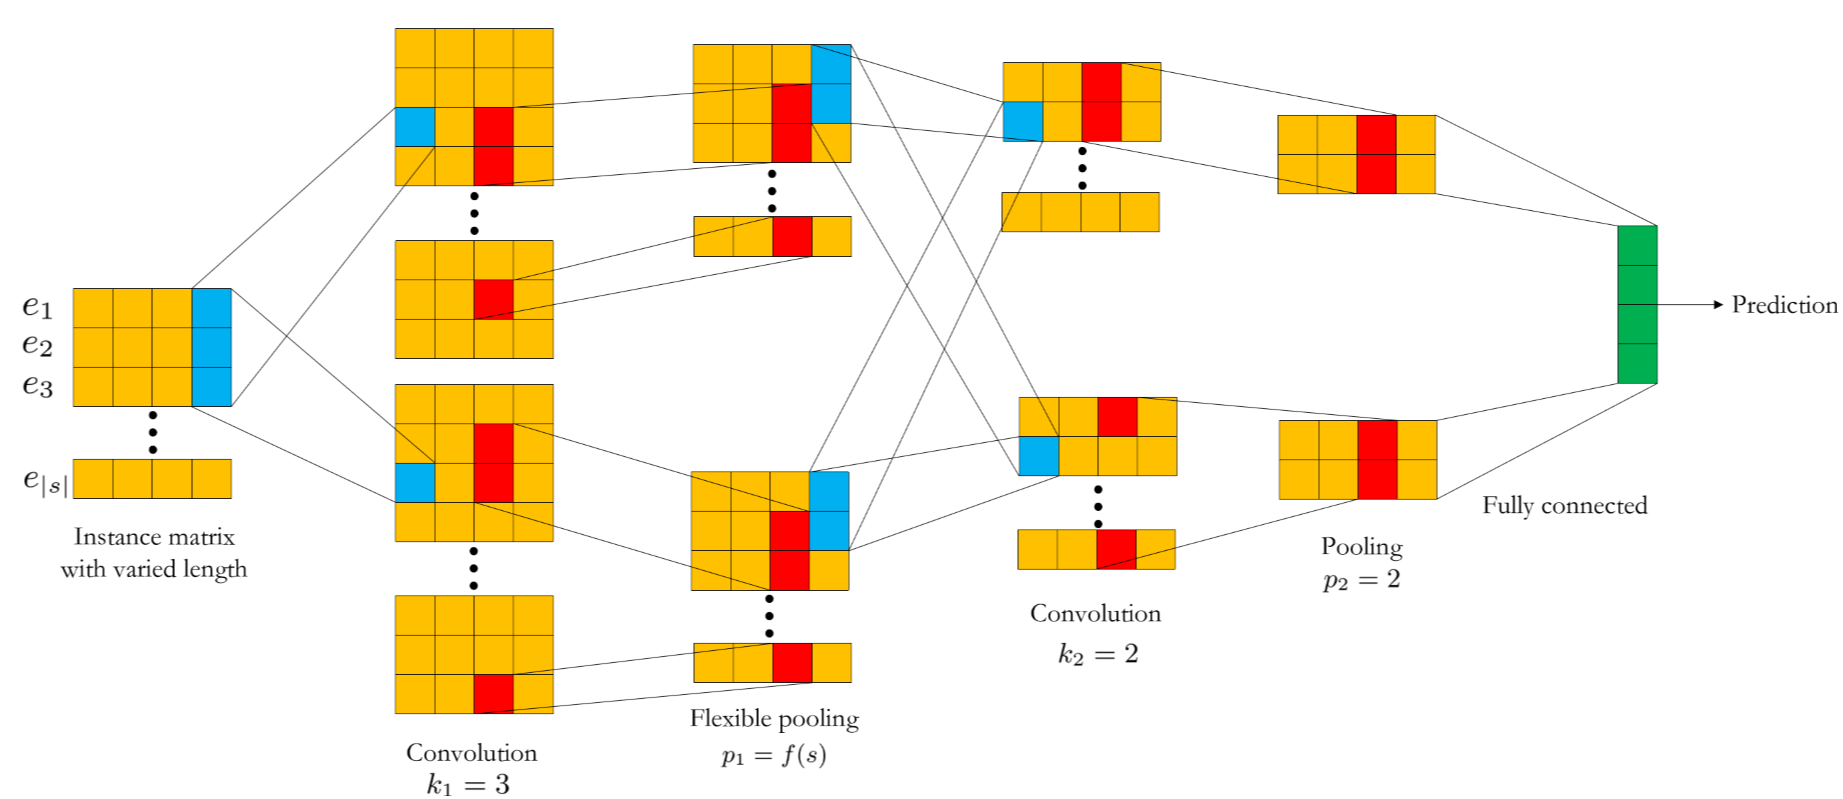
\includegraphics[width=0.8\textwidth]{../figures/ccpm}
    \caption{Convolution Click Prediction Model architecture. Source: \citep{RefWorks:liu2015convolutional}.}
    \label{fig:ccpm}
\end{figure}

The input to the CCPM model consists of a $s \times D$ dimensional matrix of stacked categorical
feature empeddigs, as shown on the left-hand side of Figure~\ref{fig:ccpm}. Per the standard
architecture discussed in \citep{RefWorks:liu2015convolutional}, this matrix is then passed through
a series of Convolutional and Pooling layers. The number
of maximum features that the intermediate pooling layers take is flexible to account for the
flexible input matrix length. The final prediction is calculated by passing the final
pooling result through a MLP, shown on the right-hand side of Figure~\ref{fig:ccpm} in green.
This makes the CCPM model a Single Tower architecture model that can be roughly summarized
as per equation~\ref{eqn:ccpm}.

\begin{equation}\label{eqn:ccpm}
    f_{\Theta}^{CCPM}(\tilde{\mathbf{x}}) = f_{\Phi}^{MLP}(f_{\Omega}^{Conv}(\tilde{\mathbf{x}}))
\end{equation}

where $f_{\Omega}^{Conv}$ represents the series of convolutions and pooling layers described above.

\cite{RefWorks:liu2015convolutional} show that the CCPM model outperforms the LR, FM and RNN models
in terms of Log Loss/Binary Cross-Entropy. However, a common critisizm of the CCPM model is that
due to the equivariance property of the Convolution operations, the degree to which it is able to capture
important feature interactions in the data is highly dependant on how the features are ordered in the
input matrix \citep{RefWorks:zhang2021deep,RefWorks:qu2018product-based,RefWorks:gu2021ad}. Convolutions
by nature extract feature maps in the local neighbourhood of each variable, but fail to do so globally.
The \textbf{Feature Generation by Convolutional Neural Network} model proposed by \cite{RefWorks:liu2019feature}.
The architecture for the FGCNN model is shown in Figure~\ref{fig:fgcnn}

\begin{figure}[h]
    \centering
    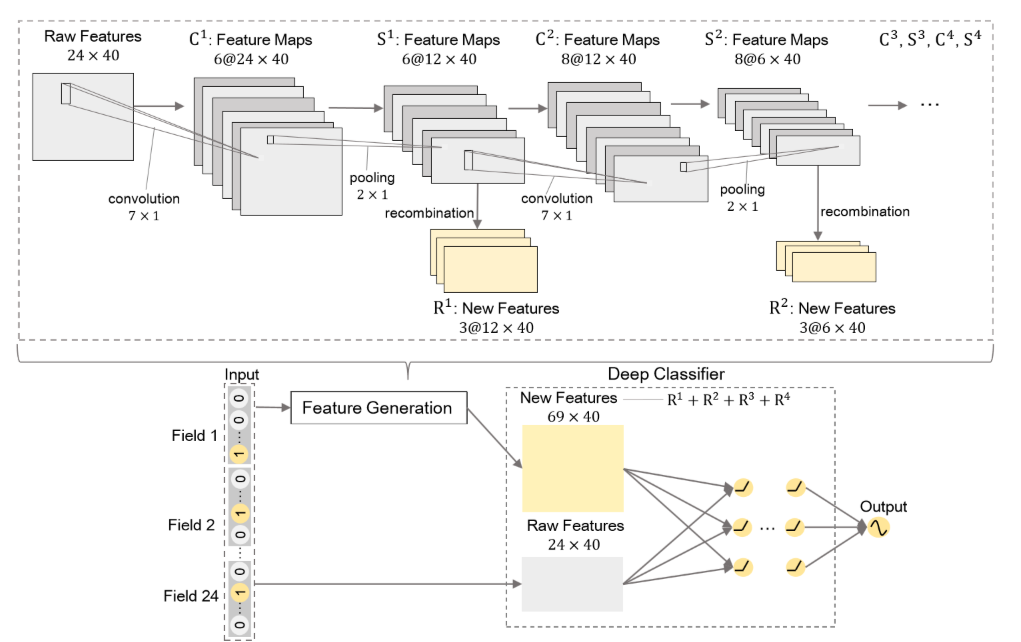
\includegraphics[width=\textwidth]{../figures/fgcnn.png}
    \caption{FGCNN model architecture with Feature Generation Component. Source: \citep{RefWorks:liu2019feature}}
    \label{fig:fgcnn}
\end{figure}

The main body of the FGCNN model consists Deep Classifier that is essentially an Inner Product
Neural Network, which was discussed above \citep{RefWorks:qu2018product-based}. The inputs
to the Deep Classifier consist of the input feature embeddings ($\tilde{\mathbf{x}}$), concatenated
with a set of new features that are created in the Feature Generation component of the model. This
Feature Generation component represents the primary innovation of the FGCNN model, and is visualized
at the top of Figure~\ref{fig:fgcnn}. As with CCPM, the Feature Generation component is composed of
a searies of two dimensional convolutional and max pooling layers, and takes the input feature
embedding matrix as an input. However, in order to solve for the input order dependancy issue
prevailent with CCPM, the resulting feature maps are first passed through a fully connected \emph{recombination layer}
that models non-adjacent interactions.

\subsubsection{Attention Operators}

\textbf{Attention Operator Models} aim to utilize the attention mechanism for identifying
the key feature interactions in the data. The \textbf{Autotomatic Feature Interaction Learning} (AutoInt) 
model proposed by \cite{RefWorks:song2019autoint} makes use of a multi-head self attention
network to model the important feature interactions in the data. The initial 
paper separates the model into three parts: an embedding layer, an interaction layer 
and an output layer. The embedding layer aims to project each sparse multi-value
categorical a and dense numerical feature into a lower dimensional space, as per the below:

$$
\mathbf{e_i} = \frac{1}{q} \mathbf{V_i x_i}
$$

where $\mathbf{V_i}$ is the embedding matrix for the $i$-th field, $x_i$ is a multi-hot vector, and $q$ 
is the number of non-zero values in $x_i$. The interaction layer employs the multi-head
mechanism to determine which higher order feature interaction are meaningful in the data. This not only
improves the efficiency of model traning, but it also improves the model's explainability. Lastly,
the output layer is a fully connected layer that takes in the concatinated output 
of the interaction layer, and applies the sigmoid activation function to produce the final prediction.
The architecture of the AutoInt model is shown in Figure\ref{fig:autoint}.

\begin{figure}[h]
    \centering
    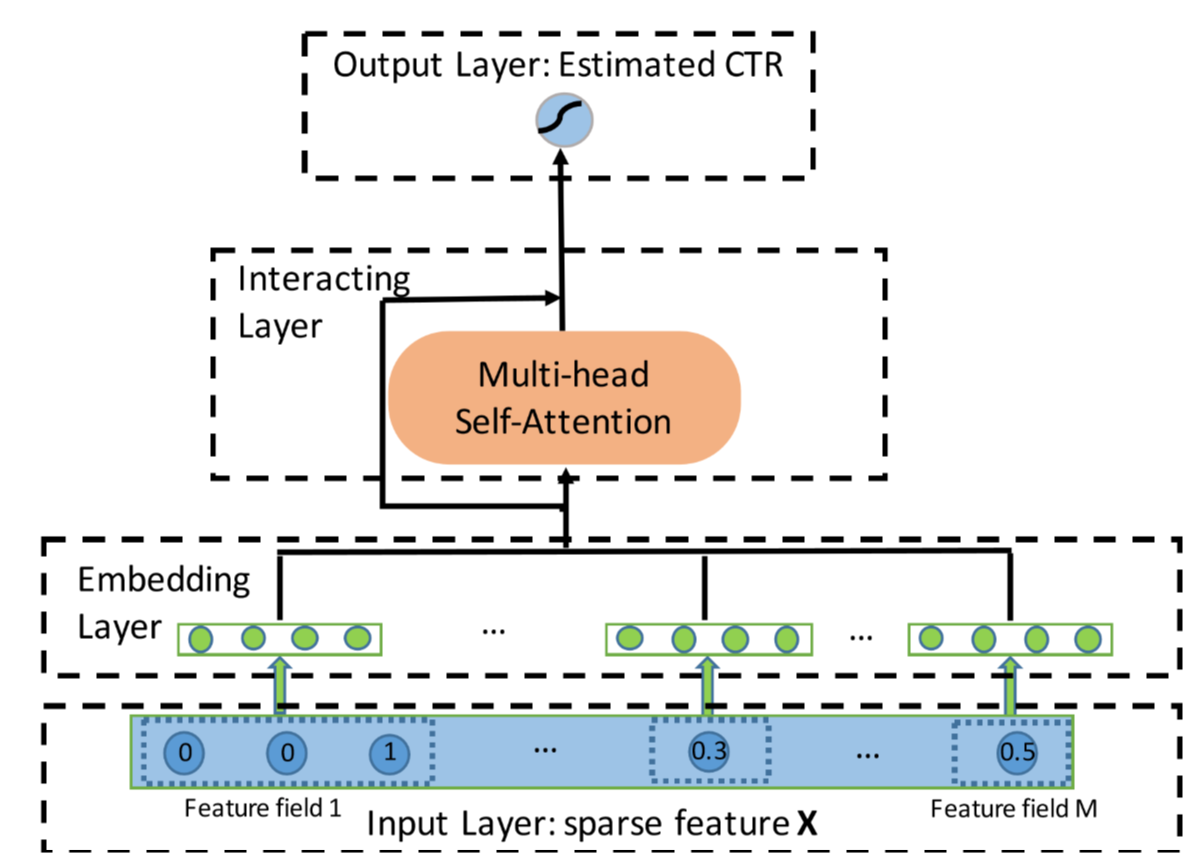
\includegraphics[width=0.8\textwidth]{../figures/autoint.png}
    \caption{The Automatic Feature Interaction Learning model architecture. Source: \citep{RefWorks:song2019autoint}}
    \label{fig:autoint}
\end{figure}


\section{Deep Reinforcement Learning}

The second part of the background chapter is dedicated to Deep Reinforcement Learning. We first
proceed by explaining the fondational concepts, in which we will establish definitions for
Markov Decision Processes, Reinforcement Learning and Dynamic Programming. We then move on to explain
Q-Learning, a specific class of Reinforcement Learning algorithms, as well as how Deep Learning
models are being applied in the case of Deep Q-Learning. Finally, we introduce the Deep Reinforcement
Learning News reccomendation (DRN) algorithm \citep{RefWorks:zheng2018drn:}, a Q-learning algorithm
which we have repurposed for ad recommendation.

\subsection{Reinforcement Learning Basics}

\subsubsection{Markov Decision Process and Bellman Optimality Equations}

In the case of many online systems and applications where there is a series of interactions between
users and the system, it is often desirable to find the optimal set of content to display to the
users in order to maximize their engagement as time goes on. This problem can be framed as a
\textbf{Markov Decision Process}. Definition~\ref{def:mdp} was taken from \citep{pike-burke2024LearnigAgents}:

\begin{definition}\label{def:mdp}
    An episodic \textbf{Markov decision process} (MDP) is defined by tuple $\mathcal{M}
    (\mathcal{S},\mathcal{A}, H,\nu, \{P_{h}\}_{h=1}^{H},\{r_{h}\}_{h=1}^{H})$ where:
    \begin{itemize}
        \item $\mathcal{S}$ is the state space of finite cardinality.
        \item $\mathcal{A}$ is the finite set of actions.
        \item $H \in \mathbb{N}$ is the horizon of the problem.
        \item $\nu$ is the initial state distribution.
        \item $\{P_{h}\}_{h=1}^{H}$ is the collection of transition functions where
        $P_h: \mathcal{S} \times \mathcal{A} \rightarrow \Delta(\mathcal{S})$
        where $\Delta(\mathcal{S})$ is the set of probability distributions over
        $\mathcal{S}$. When action $a \in \mathcal{A}$ is taken from state $s \in \mathcal{S}$
        at stage $h$, $P_h(s^\prime | s, a)$ gives the probability of transitioning to state
        $s^\prime \in \mathcal{S}$ for all $s^\prime \in \mathcal{S}$.
        \item $\{r_{h}\}_{h=1}^{H}$ is the collection of reward functions, $r_h : \mathcal{S} \times \mathcal{A} \rightarrow [0,1]$
        where $r_h(s,a)$ gives the reward from taking action $a \in \mathcal{A}$ from state $s \in \mathcal{S}$
        at stage $h \in \{1, \ldots, H\}$.
    \end{itemize}
\end{definition}

The aim of \textbf{Reinforcement Learning} is to interact with the MDP process environment in such a way
that allows the agent to learn the \emph{optimal policy} - i.e. the state-stage $\rightarrow$ action mapping
that maximizes the \emph{value} over the longer term. We refine some of these terms with more definitions
from \citep{pike-burke2024LearnigAgents} below:

\begin{definition}\label{def:policy}
    A \textbf{policy} $\pi = \{\pi_h\}_{h=1}^{H}$ is a sequence of mappings $\pi_h : \mathcal{S}
    \rightarrow \mathcal{A}$ for any $s \in \mathcal{S}, a \in \mathcal{A}$.
\end{definition}

\begin{definition}\label{def:policy-value}
    the \textbf{value} of a policy $\pi$ from state $s \in \mathcal{S}$ in stage
    $h \in \{1, \ldots, H\}$ is given by:
    \begin{equation}\label{eqn:value-function}
        V_h^{\pi} = \mathbb{E} \left[ \sum_{l = h}^{H} r_l (s_l, a_l) \Bigm| s_h = s, a_l = \pi(s_l), s_{l+1} \sim P_l(\cdot | s_l, a_l)\right]
    \end{equation}
\end{definition}

The \emph{optimal policy} $\pi^*$ is then the one with the highest value, i.e.:
\[
\pi_h^*(s) = \arg\max_{\pi \in \Pi} V_h^{\pi}(s)
\]
for any $s \in \mathcal{S}$ and any $h \in \{1,\ldots, H\}$. In order to optimize for the
policy that maximizes the expected value, we would need to consider the expected
value of taking a specific action $a$ at specific stage $h$ and state $s$, for some given policy $\pi$. This is given
by the \textbf{Q-function}, defined below in definition~\ref{def:q-function}.

\begin{definition}\label{def:q-function}
    The \textbf{Q-function} associated with taking action $a \in \mathcal{A}$ from state
    $s \in \mathcal{S}$ at stage $h \in \{1, \ldots, H\}$ under some given policy $\pi$ is given by
    \begin{equation}\label{eqn:q-function}
        Q_h^{\pi}(s,a) = \mathbb{E} \left[ \sum_{l = h}^{H} r_l (s_l, a_l) \Bigm| s_h = s, 
        a_h = a, a_l = \pi(s_l), s_{l+1} \sim P_l(\cdot | s_l, a_l)\right]
    \end{equation}
\end{definition}

The relationship between the value function $V$ and the state action value function $Q$ is
summarized in the $\textbf{Bellman equations}$. For any policy $\pi$ and for all $h, s, a$:

\begin{align*}
    V_{h}^{\pi}(s) &= Q_{h}^{\pi}(s, \pi_{h}(s))\\
    Q_{h}^{\pi}(s,a) &= r_h(s,a) + \sum_{s^\prime \in \mathcal{S}} P_h (s^\prime | s, a)V_{h+1}^{\pi}(s^\prime)\\
    V_{H+1}^{\pi}(s) &= 0
\end{align*}

The above leads to the key equations that underpin Reinforcement Learning - the \textbf{Bellman Optimality equations}.

\begin{proposition}\label{prop:bellman-optimality}
    If $V^*$ satisfies the Bellman Optimality Equations, then for all $h, a, s$:
    \begin{align*}
        V_h^*(s) &= \max_{a \in \mathcal{A}}Q_{h}^*(s,a)\\
        Q_h^*(s,a) &= r_h(s,a) + \sum_{s^\prime \in \mathcal{S}} P_h (s^\prime | s, a)V_{h+1}^*(s^\prime)\\
        V_{H+1}^*(s) = 0
    \end{align*}
    The above implies that the optimal policy $\pi^*$ is given by:
    \[
    \pi_h^*(x) = \arg\max_{a \in \mathcal{A}} Q_h^*(s,a)
    \]
\end{proposition}

In other words, the optimal policy is found by maximizing the $Q$-function at each stage and
state.

\subsubsection{Dynamic Programming and UCBRL and Thompson Sampling RL}

When the transition probabilities $P_h(s^\prime|s,a)$ and reward function
$r_h(s,a)$ are known, it is then possible to find the optimal policy by first calculating the
value of the $Q$ function at stage of the episode (which will simply be $r_H(s,a)$), and then working
back to find $Q_h^*(s,a)$ for each stage. This is known as the \emph{Dynamic Programming} or 
the \emph{Backward Recursion} algorithm. The steps involved are described in algorithm~\ref{alg:dynammic-programming}.

\begin{algorithm}
    \caption{Dynammic Programming algorithm}\label{alg:dynammic-programming}
    \begin{algorithmic}[1]
        \Require $P_h(s^\prime|s,a)$ and $r_h(s,a)$ are known
        \State Set $V_{H+1}^*(s) = 0$ for all $s \in \mathcal{S}$
        \For{$h = H, \ldots, 1$}
            \State Calculate $Q_h^*(s,a) = r_h(s,a) + \sum_{s^\prime \in \mathcal{S}}P_h(s^\prime |s,a) V_{h+1}^*(s^\prime)$
            \State Set $\pi_h^*(s) = \arg\max_{a \in \mathcal{A}} Q_h^*(s,a)$
            \State Define $V_h^*(s) = \max_{a \in \mathcal{A}}Q_h^*(s,a) = Q_h^*(s, \pi_h^*(s))$
        \EndFor
    \end{algorithmic}
\end{algorithm}

\subsection{Q-Learning and Deep Q-Learning}

\subsection{DRN: Deep Reinforcement Learning for News Recommendation}

In their survey, \citep{RefWorks:wang2024deep} describe how deep reinforcement learning combines 
the aforementioned feature extraction capabilities of DNN’s with the decision-making 
capability of reinforcement learning, which aims to learn an optimal state-action policy 
which maximizes the expected reward gained in a given environment. In the context of 
recommendation systems, a significant amount of research has been dedicated to formulating 
the recommendation problem as a Contextual Multi-Armed Bandit (MAB) problem setting, where 
the context consists of user, site and item features \citep{RefWorks:bouneffouf2012contextual-bandit,RefWorks:li2010contextual-bandit,RefWorks:zeng2016online}. 
However, a shortcoming for the MAB approach 
is that it does not explicitly model the future expected reward for the policy, which may 
be detrimental in the longer term \citep{RefWorks:zheng2018drn:}. Markov Decision Process (MDP) models 
solve for this issue by modelling the state-action progression as a Markov Process, allowing 
for the stochastic valuation of the future potential rewards for a given recommendation 
policy \citep{RefWorks:lu2016partially,RefWorks:mahmood2007learning}. DRN \citep{RefWorks:zheng2018drn:} is a MDP framework 
that leverages a Deep Neural Network to approximate the expected total user response for 
each recommendation at each state. The two major advantages of DRN are firstly that it is 
composed on the basis of a continuous state and action representation, meaning that it can 
be scaled to large and sparse datasets, and secondly that the proposed reward function 
consists of both the immediate reward (user click) as well as the future expected reward 
(long term user engagement), thereby allowing for better recommendations over a user’s 
lifetime.

\chapter{Deep CTR model Evaluation}
\label{chap:deep-ctr-model-evaluation}

\section{Model Selection Methodology}

As explained above, I will explore a number of deep learning models. I selected five popular models on the basis of the following criteria

\begin{itemize}
\item Competitive predition accuracy in the KDD12, Criteo and Avazu datasets as published on Papers with Code.
\item Ideally, I was looking for a representitive set of models for each model type as discussed in (Zhang et. al. 2021). Therefore I was looking for models that employed Product Interaction Opetators, Attention Operators and Factorization Machines as a basis.
\item The code for the model has to be accessible and intuitive to use.
\end{itemize}

On the basis of the above critea, I have chosen the following models to explore:

\begin{itemize}
\item Factorization Supported Neural Networks
\item Product Based Neural Networks
\item Wide and Deep
\item DeepFM
\item Automatic Feature Interaction (AutoInt)
\end{itemize}

\section{Experiment Setup}

\subsection{Datasets and Preprocessing}

\subsection{Evaluation Metrics}

\subsection{Hyperparameter Selection}

\section{Deep CTR Model Results}

\chapter{Deep Reinforcement Learning for Ad Personalization}
\label{chap:deep-rl-for-ad-personalization}

\section{DeepCTR-RL Framework}

\subsection{Model Framework}

\subsection{Feature types}

\subsection{Double Deep Q-Learning Network}

\subsection{Exploration}

\subsection{Experience Replay}

\section{Experiment Setup}

\subsection{Dataset and Preprocessing}

\subsection{Evaluation Metrics}

\subsection{Hyperparameter Selection}

\section{Deep CTR-RL Results}

\chapter{Discussion}
\label{chap:discussion}

Discussion goes here.

\chapter{Conclusion}


Conclusion goes here. 





\clearpage
 %% reset page counter and start appendix pages with A
\pagenumbering{arabic}
\renewcommand*{\thepage}{A\arabic{page}}

%% Appendix goes here
\appendix
%
\chapter{Appendix}

\section{Abbreviations and Acronyms}
\label{app:acronyms}

\begin{table}[ht]
    %\centering
    \begin{tabular}{|l|l|l|}
      \hline
        \textbf{Term} & \textbf{Definition} & \textbf{Reference} \\
      \hline
        LR& Logistic Regression & \\
        FM & Factorization Machine & \\
        FFM & Field-Aware Factorization Machine & \\
        DNN & Deep Neural Network & \\
        MLP & Multilayer Perceptron & \ref{ref:mlp} \\
    \hline
    \end{tabular}
\end{table}


\section{Notation}
\label{app:notation}

\begin{table}[ht]
    %\centering
    \begin{tabular}{|l|l|l|}
      \hline
        \textbf{Symbol} & \textbf{Definition} & \textbf{Reference} \\
      \hline
        $\mathbf{x}$& Feature vector, before pre-processing &\\
        $n$ & the number of features in $\mathbf{x}$ &\\
        $x_i$& The $i$-th feature in $\mathbf{x}$ &\\
        $\mathbf{x_i}^{OH}$ & One-hot encoded vector representation of categorical feature $i$ &\\
        $\mathbf{e}_i$ & Embedded vector representation of categorical feature $i$ & \\
        $z_i$ & Mean and variance standardized value for feature $i$ from $\mathbf{x}$ &\\
        $\tilde{\mathbf{x}}$ & $\mathbf{x}$ after catigorical embedding and numerical standardization. &\\
        $f$ & Pre-sigmoid classification function &\\
        $\Theta$ & Parameter vector for $f$ & \\
    \hline
    \end{tabular}
\end{table}


%%References part of appendices
% References: modify the file refs.bib
\bibliographystyle{plainnat}
\bibliography{refs}


\end{document}
